% This LaTeX was auto-generated from MATLAB code.
% To make changes, update the MATLAB code and export to LaTeX again.

\documentclass{article}

\usepackage[utf8]{inputenc}
\usepackage[T1]{fontenc}
\usepackage{lmodern}
\usepackage{graphicx}
\usepackage{color}
\usepackage{hyperref}
\usepackage{amsmath}
\usepackage{amsfonts}
\usepackage{epstopdf}
\usepackage[table]{xcolor}
\usepackage{matlab}

\sloppy
\epstopdfsetup{outdir=./}
\graphicspath{ {./LASK_images/} }

\begin{document}

\matlabtitle{\textbf{Amplititude-shift keying trasmitter}}

\begin{matlabcode}
clear all % clear all varables
close all % close all plots
clc % clear the screen in the command window
warning('off','all')

\end{matlabcode}

\begin{par}
\begin{center}
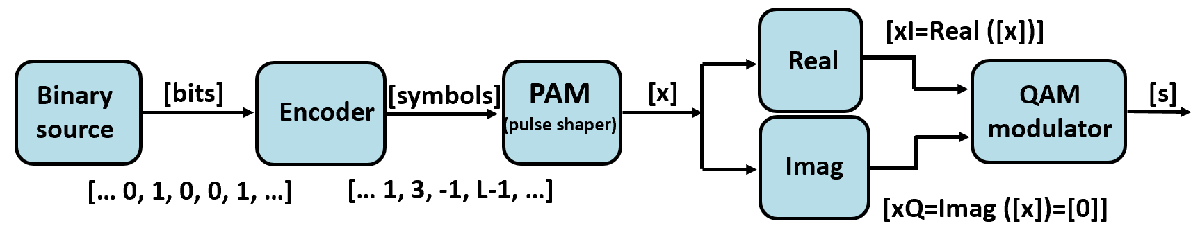
\includegraphics[width=\maxwidth{73.55745107877571em}]{image_0}
\end{center}
\end{par}

\begin{par}
\begin{flushleft}
ASK is an amplitude modulation that tranform digital data to fixed-amplitude carrier wave at fixed frequency.The picture above shows the inplemented system process. Binary source is encoded form bits to symbols by encouder and shaped into viarous amplitude pluse by PAM. L-ASK singals do not have any in quadrature components, So take the output of PAM and feed it into the QAM in-phase signal input of the QAM modulation system.This is the inplemented modulation system.
\end{flushleft}
\end{par}

\begin{par}
\begin{flushleft}
\textbf{ Setting signal specifications}
\end{flushleft}
\end{par}

\begin{matlabcode}
%----------------------------------------------------------------
% *Signal specifications*
bits_per_symbol=2; % number of bits that correspond to a symbol
L=2^bits_per_symbol; % number of levels of the modulation alphabet
nbits=1000*bits_per_symbol; % number of bits to be transmitted
Br=1000; % [bits/s] bit rate
fs=50000; % [samples/s] sampling frequency
fc=3000; % [Hz] carrier frequency
Bs=Br/log2(L); % [symbols/s] Symbol rate
nsps=fs/Bs; % samples per symbol
%----------------------------------------------------------------
\end{matlabcode}

\begin{par}
\begin{flushleft}
\textbf{The Pluse shaper}
\end{flushleft}
\end{par}

\begin{par}
\begin{flushleft}
we have two different plusetypes \textbf{ROOTRAISEDCOSINE} and \textbf{RECT}
\end{flushleft}
\end{par}

\begin{par}
\begin{center}
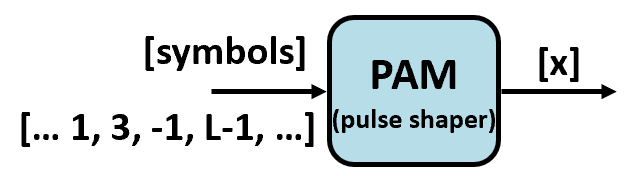
\includegraphics[width=\maxwidth{40.642247867536376em}]{image_1}
\end{center}
\end{par}

\begin{matlabcode}
% *Pulse shaper specifications*
Nf=5*nsps; % number of filter coefficients (=five time the symbol duration)
pulsetype='ROOTRAISEDCOSINE'; % pulsetype: 'RECT' or 'ROOTRAISEDCOSINE'
switch pulsetype
case 'ROOTRAISEDCOSINE'
rolloff=0.8; % roll-off factor for root raised cosine pulses
bandwidth_Hz=0.5*Bs*(1+rolloff) % bandwidth of the baseband signal
case 'RECT'
rolloff=[];
bandwidth_first_lobe_Hz=Bs;
end
\end{matlabcode}
\begin{matlaboutput}
bandwidth_Hz = 450
\end{matlaboutput}
\begin{matlabcode}
%----------------------------------------------------------------
\end{matlabcode}

\begin{par}
\begin{flushleft}
\textbf{Binary source}
\end{flushleft}
\end{par}

\begin{par}
\begin{center}
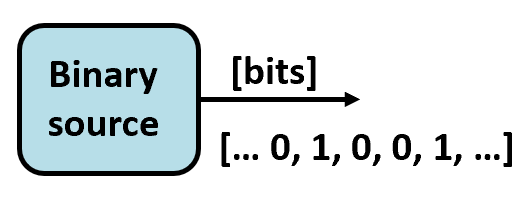
\includegraphics[width=\maxwidth{28.499749121926744em}]{image_2}
\end{center}
\end{par}

\begin{par}
\begin{flushleft}
Using function BinarySource\_2023() generate nbits binary bits
\end{flushleft}
\end{par}

\begin{par}
\begin{flushleft}
The function BinarySource\_2023() using Matlab function randi generate 1 by nbits matrix to describe the binary source
\end{flushleft}
\end{par}

\begin{matlabcode}
% *Source bits generation*
source_bits=BinarySource_2023(nbits); % vector with the source bits
\end{matlabcode}

\begin{par}
\begin{flushleft}
\textbf{Encoder}
\end{flushleft}
\end{par}

\begin{par}
\begin{center}
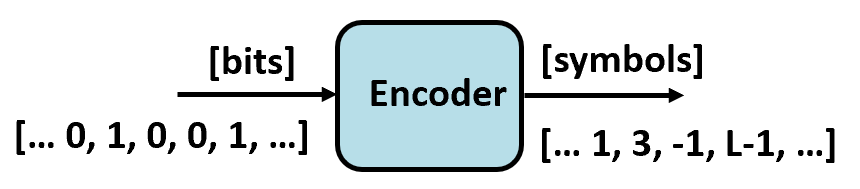
\includegraphics[width=\maxwidth{46.362267937782235em}]{image_3}
\end{center}
\end{par}

\begin{par}
\begin{flushleft}
The Encoder\_2023() function given as input a victior of bit source bits, generate as output a victior of symbols using the multi-level symmetric alphabet \{-1,1,-3,3... -L+1,L-1\}  of L=nlevels levels(L=2,4,8),according the Gray rule.
\end{flushleft}
\end{par}

\begin{matlabcode}
%----------------------------------------------------------------
% *Symbols generation with Gray mapping*
symbols=Encoder_2023(source_bits, L);
\end{matlabcode}
\begin{matlaboutput}
bit_table = 4x2    
     0     0
     0     1
     1     1
     1     0

symbol_table = 4x1    
    -3
    -1
     1
     3

\end{matlaboutput}

\begin{par}
\begin{flushleft}
\textbf{Plot of the constellation}
\end{flushleft}
\end{par}

\begin{matlabcode}
%----------------------------------------------------------------
% *Plot of the constellation*
figure
plot(real(symbols),imag(symbols),'o','MarkerFaceColor','r'),
axis ([-L+1 L-1 -L+1 L-1]);
title('Constellation');
xlabel('in-phase');
ylabel('quadrature');
\end{matlabcode}
\begin{center}
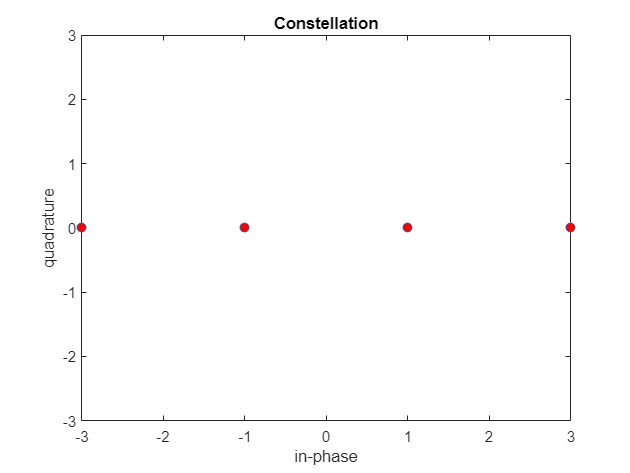
\includegraphics[width=\maxwidth{56.196688409433015em}]{figure_0.png}
\end{center}

\begin{par}
\begin{flushleft}
The picture above shows the constellation of QAM signals, with x-axis representing in phase signals and y-axis representing quadrature signals, which leads to the conclusion that L-ASK signals do not have any quadrature components.
\end{flushleft}
\end{par}

\begin{par}
\begin{flushleft}
\textbf{Generation of the baseband PAM signal}
\end{flushleft}
\end{par}

\begin{matlabcode}
%----------------------------------------------------------------
% *Generation of the baseband PAM signal*
x=PAMmodulator_2023(symbols,nsps,Nf,pulsetype,rolloff);
Ts=1/fs;% sampling interval
T=Ts*(length(x)-1); % signal duration
%----------------------------------------------------------------
% *Plot of the baseband PAM signal and of its spectrum*
figure
t=0:1/fs:T;
plot(t,x)
xlabel('t [s]')
ylabel ('[V]')
title('PAM signal')
axis([min(t) max(t) 1.2*min(x) 1.2*max(x)])
\end{matlabcode}
\begin{center}
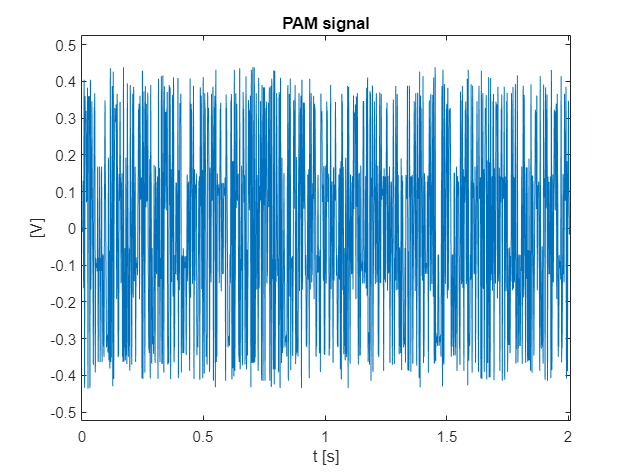
\includegraphics[width=\maxwidth{56.196688409433015em}]{figure_1.png}
\end{center}
\begin{matlabcode}
figure
PlotSpectrum_2023(x,fs);
title('Spectrum of the PAM signal')
\end{matlabcode}
\begin{center}
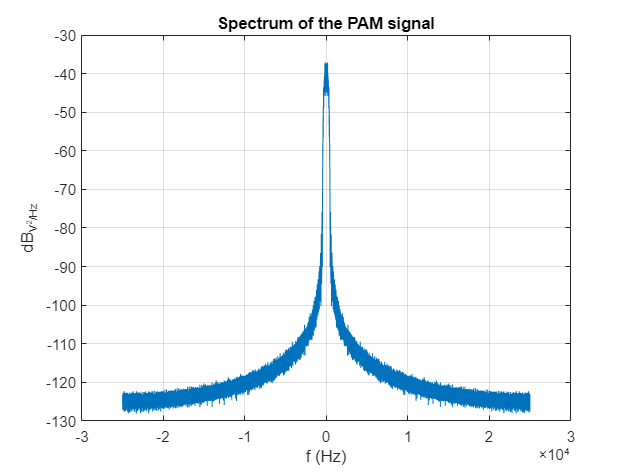
\includegraphics[width=\maxwidth{56.196688409433015em}]{figure_2.png}
\end{center}


\vspace{1em}
\begin{par}
\begin{flushleft}
\textbf{QAM modulator}
\end{flushleft}
\end{par}

\begin{par}
\begin{center}
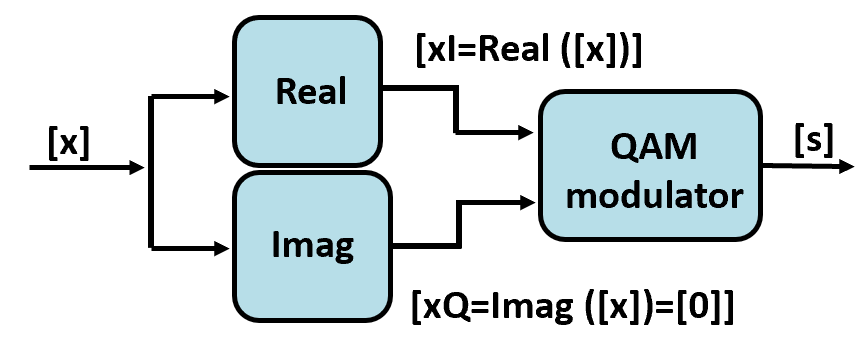
\includegraphics[width=\maxwidth{70.24586051179126em}]{image_4}
\end{center}
\end{par}

\begin{matlabcode}
% *L-ASK modulation through the QAM modulator*
xI=x % in-phase signal
\end{matlabcode}
\begin{matlaboutput}
xI = 1x100500    
   -0.0002   -0.0003   -0.0004   -0.0005   -0.0006   -0.0007   -0.0008   -0.0009   -0.0010   -0.0011   -0.0012   -0.0013   -0.0014   -0.0014   -0.0015   -0.0016   -0.0017   -0.0018   -0.0019   -0.0019   -0.0020   -0.0021   -0.0021   -0.0022   -0.0022   -0.0023   -0.0023   -0.0023   -0.0023   -0.0024   -0.0024   -0.0024   -0.0024   -0.0024   -0.0024   -0.0023   -0.0023   -0.0023   -0.0022   -0.0022   -0.0021   -0.0020   -0.0020   -0.0019   -0.0018   -0.0017   -0.0016   -0.0015   -0.0014   -0.0013

\end{matlaboutput}
\begin{matlabcode}
xQ=zeros(1,length(x)) % the quadrature component is zero
\end{matlabcode}
\begin{matlaboutput}
xQ = 1x100500    
     0     0     0     0     0     0     0     0     0     0     0     0     0     0     0     0     0     0     0     0     0     0     0     0     0     0     0     0     0     0     0     0     0     0     0     0     0     0     0     0     0     0     0     0     0     0     0     0     0     0

\end{matlaboutput}
\begin{matlabcode}
s=ModQAM_2023(xI,xQ,fc,T,fs);
%----------------------------------------------------------------
% *Plot of the L-ASK signal and of its spectrum*
figure
plot(t,s,'r')
hold on
plot(t,x,'b')
axis([min(t) max(t) 1.2*min(x) 1.2*max(x)])
xlabel('t [s]')
ylabel ('[V]')
title('L-ASK signal')
legend('L-ASK signal','PAM signal')
\end{matlabcode}
\begin{center}
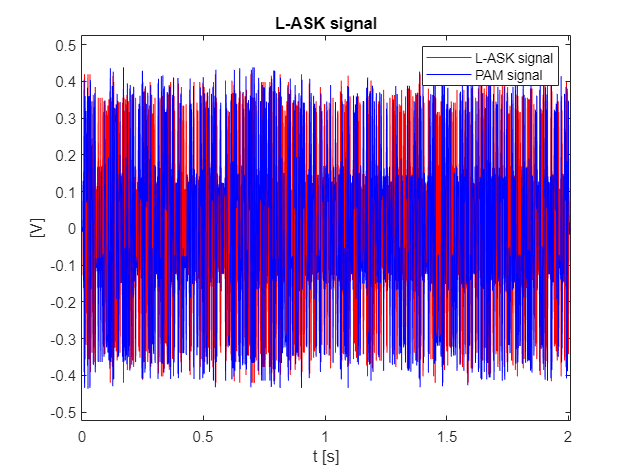
\includegraphics[width=\maxwidth{56.196688409433015em}]{figure_3.png}
\end{center}
\begin{matlabcode}
figure
PlotSpectrum_2023(s,fs);
title('Spectrum of the modulated signal')
\end{matlabcode}
\begin{center}
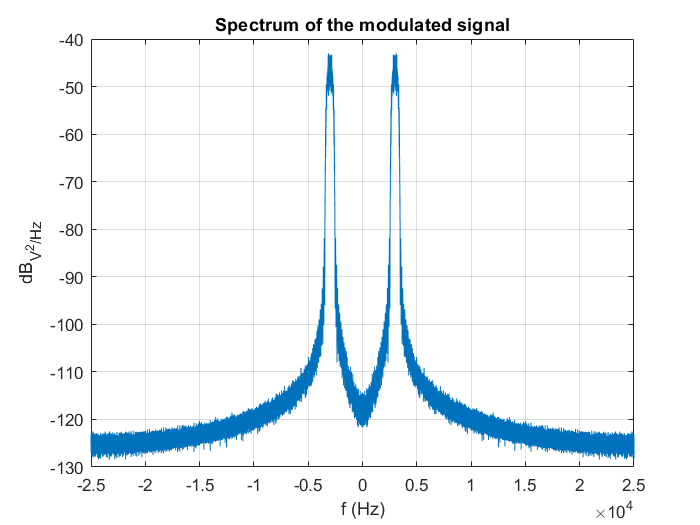
\includegraphics[width=\maxwidth{56.196688409433015em}]{figure_4.png}
\end{center}
\begin{matlabcode}
%----------------------------------------------------------------
% output the signal to the audio card
sound(s,fs)
\end{matlabcode}

\end{document}
